\documentclass[12pt,a4paper]{article}

% ── Packages ──────────────────────────────────────────────────────
\usepackage[margin=2.5cm,headheight=14pt]{geometry}
\usepackage{graphicx}
\usepackage{hyperref}
\usepackage{xcolor}
\usepackage{titlesec}
\usepackage{fancyhdr}
\usepackage{booktabs}
\usepackage{longtable}
\usepackage{tabularx}
\usepackage{enumitem}
\usepackage{listings}
\usepackage{float}
\usepackage{caption}
\usepackage{tikz}
\usetikzlibrary{shapes.geometric, arrows.meta, positioning, fit, backgrounds, calc}
\usepackage{tocloft}
\usepackage{parskip}
\usepackage[T1]{fontenc}
\usepackage{lmodern}
\usepackage{microtype}

% ── Colours ───────────────────────────────────────────────────────
\definecolor{oghmablue}{HTML}{1E3A5F}
\definecolor{oghmaaccent}{HTML}{3B82F6}
\definecolor{codebg}{HTML}{F5F5F5}
\definecolor{linkblue}{HTML}{2563EB}

% ── Diagram colours ──────────────────────────────────────────────
\definecolor{decisionamber}{HTML}{D97706}
\definecolor{storeteal}{HTML}{0D9488}
\definecolor{queueviolet}{HTML}{7C3AED}
\definecolor{errorred}{HTML}{DC2626}
\definecolor{homelabgreen}{HTML}{059669}
\definecolor{externalamber}{HTML}{B45309}

% ── Hyperref config ───────────────────────────────────────────────
\hypersetup{
    colorlinks=true,
    linkcolor=black,
    urlcolor=oghmablue,
    citecolor=black,
    pdfauthor={Semyon Fox, Samuel Regan, Shreyansh Singh},
    pdftitle={OghmaNotes -- CT216 Project Report},
}

% ── Header/Footer ─────────────────────────────────────────────────
\pagestyle{fancy}
\fancyhf{}
\fancyhead[L]{\small\textcolor{oghmablue}{OghmaNotes}}
\fancyhead[R]{\small\textcolor{oghmablue}{CT216 Software Engineering I}}
\fancyfoot[C]{\thepage}
\renewcommand{\headrulewidth}{0.4pt}

% ── Section formatting ────────────────────────────────────────────
\titleformat{\section}
    {\Large\bfseries\color{oghmablue}}{\thesection}{1em}{}[\vspace{-0.5em}\textcolor{oghmaaccent}{\rule{\textwidth}{0.8pt}}]
\titleformat{\subsection}
    {\large\bfseries\color{oghmablue}}{\thesubsection}{1em}{}
\titleformat{\subsubsection}
    {\normalsize\bfseries\color{oghmablue}}{\thesubsubsection}{1em}{}

% ── Code listing style ────────────────────────────────────────────
\lstset{
    backgroundcolor=\color{codebg},
    basicstyle=\small\ttfamily,
    breaklines=true,
    frame=single,
    rulecolor=\color{gray},
    numbers=left,
    numberstyle=\tiny\color{gray},
    tabsize=2,
    showstringspaces=false,
}

% Screenshot command: \screenshot{filename}{caption}
\newcommand{\screenshot}[2]{%
    \begin{figure}[H]
    \centering
    \IfFileExists{screenshots/#1.png}{%
        \includegraphics[width=0.9\textwidth]{screenshots/#1.png}%
    }{%
        \fbox{\parbox{0.85\textwidth}{\centering\vspace{1.5cm}\textcolor{gray}{\textit{Save as: screenshots/#1.png}}\vspace{1.5cm}}}%
    }
    \caption{#2}
    \end{figure}
}

% ── Custom commands ───────────────────────────────────────────────
\newcommand{\todo}[1]{\textcolor{red}{\textbf{[TODO: #1]}}}
\newcommand{\screenshotplaceholder}[1]{%
    \begin{figure}[H]
    \centering
    \fbox{\parbox{0.85\textwidth}{\centering\vspace{2cm}\textcolor{gray}{\textit{Screenshot: #1}}\vspace{2cm}}}
    \caption{#1}
    \end{figure}
}
\newcommand{\tech}[1]{\texttt{#1}}

% ══════════════════════════════════════════════════════════════════
\begin{document}

% ── Cover Page ────────────────────────────────────────────────────
\thispagestyle{empty}
\begin{center}
    \vspace*{2cm}

    {\Huge\bfseries\textcolor{oghmablue}{OghmaNotes}}\\[0.5cm]
    {\Large\textcolor{oghmaaccent}{AI-Powered Note-Taking with RAG \& Canvas LMS Integration}}

    \vspace{1.5cm}
    \textcolor{oghmaaccent}{\rule{0.6\textwidth}{1.5pt}}
    \vspace{1.5cm}

    {\Large\textbf{CT216: Software Engineering I}}\\[0.3cm]
    {\large Project Report}\\[0.3cm]
    {\large Academic Year 2025/2026}

    \vspace{2cm}

    \begin{tabular}{ll}
        \textbf{Semyon Fox}      & 24495896 \\
        \textbf{Samuel Regan}    & 24498764 \\
        \textbf{Shreyansh Singh} & 24316243 \\
    \end{tabular}

    \vspace{1.5cm}

    {\large Lecturer: \textbf{Enda Barrett}}\\[0.3cm]
    {\large University of Galway}

    \vspace{1.5cm}

    \begin{tabular}{rl}
        \textbf{Live Application:} & \url{https://oghmanotes.ie} \\
        \textbf{GitHub Repository:} & \url{https://github.com/semyonfox/oghma} \\
    \end{tabular}

    \vfill
    {\large April 2026}
\end{center}
\newpage

% ── Table of Contents ─────────────────────────────────────────────
\thispagestyle{empty}
\tableofcontents
\newpage
\setcounter{page}{1}

% ══════════════════════════════════════════════════════════════════
% SECTION 1: PROJECT OVERVIEW
% ══════════════════════════════════════════════════════════════════
\section{Project Overview}
\label{sec:overview}

\subsection{Problem Statement}

University students' course content is scattered across LMS platforms, local folders, and personal notes. Tools like Notion and Obsidian have strong editors but treat uploaded documents as opaque files: users can't query their content semantically. Dedicated AI tools can answer questions but lack persistent knowledge bases scoped to a student's own materials. In practice this means searching through dozens of lecture PDFs to find a single concept, cross-referencing handwritten notes against slides in a separate window, or hunting for an assignment brief buried somewhere in a Canvas module. Nothing bridges the gap between a personal note-taking workspace and AI-powered retrieval over lecture content, integrated with the institution's LMS.

\subsection{Our Solution}

OghmaNotes is an AI-powered note-taking platform built for students. It gives users a single workspace to create and organise notes in a VSCode-inspired editor, import course materials from Canvas LMS, and query their entire knowledge base through a Retrieval-Augmented Generation (RAG) chat interface.

The platform is built with Next.js~16.2 on the frontend, a PostgreSQL database with the \tech{pgvector} extension for vector similarity search, and a suite of AWS services (RDS, S3, SQS, ECS Fargate, SES, Amplify) for production-grade infrastructure. It is live at \url{https://oghmanotes.ie}.

\subsection{Key Differentiators}

What sets it apart is RAG-powered search over notes and PDFs using semantic retrieval rather than keyword matching, direct Canvas LMS integration with one-click course import handled by a self-scaling worker, and a full AWS production stack built to real-world cloud engineering standards. The app also supports 12 languages through a custom internationalisation system.


% ══════════════════════════════════════════════════════════════════
% SECTION 2: TEAM ROLES & CONTRIBUTIONS
% ══════════════════════════════════════════════════════════════════
\section{Team Roles \& Contributions}
\label{sec:team}

Three members, each owning distinct areas of the project, over seven months of development (September 2025 -- April 2026).

\subsection{Semyon Fox --- Tech Lead / Full-Stack / DevOps}

Led the technical side of the project: system architecture, infrastructure decisions, and the majority of feature development. Key contributions include:

\begin{itemize}[leftmargin=1.5em]
    \item \textbf{Architecture \& Infrastructure:} Designed and implemented AWS infrastructure including Amplify hosting, SQS job queues, ECS Fargate workers, and ElastiCache. Made all major architectural decisions including the BullMQ to SQS migration and embedding pipeline iterations.
    \item \textbf{Frontend:} Built the VSCode-style note editor UI, file tree, command palette, settings page, Canvas import UI, and AI chat interface. Implemented internationalisation across 12 languages.
    \item \textbf{Backend:} Developed API routes for notes CRUD, file upload, AI chat with RAG, and auth middleware with rate limiting.
    \item \textbf{DevOps:} Configured Amplify CI/CD pipeline, ECS Fargate worker deployment, and environment management across dev/main/production branches.
    \item \textbf{Canvas Integration:} Built the full Canvas LMS import pipeline from API integration through to S3 storage and RAG embedding.
\end{itemize}

\subsection{Samuel Regan --- Authentication / RAG Pipeline}
Contributed to the authentication system, RAG pipeline, and frontend:
\begin{itemize}[leftmargin=1.5em]
    \item \textbf{Authentication:} Built the login and registration UI, implemented password reset with Nodemailer (later migrated to AWS SES), and developed JWT-based session tokens with middleware-based route protection across the application.
    \item \textbf{Database:} Designed the original schema for the embeddings and chunks tables, later extended this to track worker state.
    \item \textbf{RAG Pipeline:} Implemented the full ingestion flow including PDF text extraction, text chunking, embedding generation, and pgvector similarity search. Designed an asynchronous job queue with a PostgreSQL jobs table to separate document ingestion from the upload request, avoiding timeout failures on large imports. The chat prompt construction and HNSW indexing were later extended by the rest of the team.
    \item \textbf{Frontend:} Contributed targeted fixes to the file rename and zoom functionality.
\end{itemize}

\subsection{Shreyansh Singh --- Infrastructure / OAuth / Canvas API}

Contributed to the cloud infrastructure setup, authentication, and Canvas LMS integration:

\begin{itemize}[leftmargin=1.5em]
    \item \textbf{Infrastructure:} Designed and provisioned core AWS services including RDS (PostgreSQL), S3 (object storage), and SES (transactional email). Configured security groups, IAM policies, and SSL certificates for database connectivity.
    \item \textbf{Database:} Designed the PostgreSQL schema under the \tech{app} namespace (e.g.\ \tech{app.login}, \tech{app.notes}, \tech{app.chunks}), making decisions around table structure, relationships, and the use of \tech{pgvector} for embedding storage.
    \item \textbf{OAuth:} Implemented Google and GitHub OAuth flows using Auth.js (NextAuth), including provider registration, callback handling, and account linking logic.
    \item \textbf{Canvas API Integration:} Integrated the Canvas LMS REST API, covering course and file retrieval from university Canvas instances.
\end{itemize}

% ══════════════════════════════════════════════════════════════════
% SECTION 4: CUSTOMER-FACING FEATURES
% ══════════════════════════════════════════════════════════════════
\section{Customer-Facing Features}
\label{sec:features}

\subsection{Landing Page}

The landing page at \url{https://oghmanotes.ie} features a hero section, feature cards, team information, and authentication entry points. Built with Next.js App Router and Tailwind CSS~v4.

\screenshot{landing-hero}{Landing Page --- Hero section with tagline and call-to-action}

\screenshot{landing-features}{Landing Page --- Core feature cards}

\subsection{Authentication}
\label{sec:feat-auth}

OghmaNotes supports email/password registration (with SES-based email verification and password reset) and OAuth~2.0 via Google and GitHub using Auth.js. Email verification is required before access is granted --- the platform runs a live AI pipeline with real inference costs, so unverified throwaway accounts would expose it to abuse. Accounts are deduplicated by email, and rate limiting is applied to all auth endpoints. The full authentication flow is detailed in Section~\ref{sec:flow-auth}.

\screenshot{login}{Login Page --- Email/password form with Google and GitHub OAuth}

\screenshot{register}{Registration Page --- Account creation form with OAuth options}

\subsection{Notes Editor}
\label{sec:feat-editor}

The editor builds on the Notea foundation (S3-backed markdown storage), modernised and extended as described in Section~\ref{sec:pivot-1}. It uses a VSCode-inspired three-panel layout: a file tree sidebar (Obsidian-style with indent guides), a main editor pane (Lexical rich-text with CodeMirror for markdown source), and an optional split-pane PDF viewer for side-by-side study. File management covers create, rename, delete, duplicate, drag-and-drop upload, breadcrumb navigation, and a keyboard-accessible command palette.

\screenshot{notes-editor}{Notes Editor --- VSCode-inspired layout with Canvas course file tree and icon navigation}

\screenshot{search-modal}{Notes Editor --- Search modal with keyword and semantic results across imported notes}

\subsection{Canvas LMS Integration}
\label{sec:feat-canvas}

Users enter their Canvas API token and institution URL in settings. The token is encrypted at rest and decrypted at runtime for Canvas REST API calls. Users browse their courses and pick which to import. The import runs asynchronously via SQS and an ECS Fargate worker (see Section~\ref{sec:flow-canvas}).

\screenshot{canvas-settings}{Canvas Integration --- Settings page with API token configuration and connected institution}

\screenshot{canvas-import}{Canvas Import --- Course selection with active import progress and per-course status}

\subsection{Search}

Notes and imported documents are searchable via two complementary modes. Keyword search performs fast pattern matching against note titles and content. Semantic search embeds the query using \tech{mxbai-embed-large} and retrieves the most relevant notes by cosine similarity via pgvector. Both modes support filtering by Canvas course, allowing students to scope searches to a specific module. The two modes run as separate requests and results are deduplicated client-side.

\subsection{AI Chat (RAG-Powered)}
\label{sec:feat-chat}

Users ask natural-language questions about their notes and imported documents. The system embeds the query, retrieves relevant chunks via pgvector, reranks them, and streams a cited answer from the LLM. Search can be scoped to specific files or folders, sessions persist across visits, and responses can be rated with a thumbs up or down. The full pipeline is in Section~\ref{sec:flow-rag}.

\screenshot{chat}{AI Chat --- RAG-powered chat with cited responses, thinking mode, and session history}

\subsection{Settings}

The settings page provides profile management, dark mode, language selection (13 locales), Canvas API token configuration, OAuth account linking, and full vault export. The vault export streams all notes as Markdown files in a ZIP archive, preserving the folder hierarchy, with no proprietary format lock-in.

\screenshot{settings}{Settings Page --- Profile, dark theme, language selection, Canvas configuration, and data export}

\subsection{Quiz System (Spaced Repetition)}
\label{sec:feat-quiz}

OghmaNotes includes a flashcard quiz system using the FSRS (Free Spaced Repetition Scheduler) algorithm via \tech{ts-fsrs}. Users create flashcards from their notes and study with spaced-repetition scheduling tuned for long-term retention. The system tracks quiz sessions, individual card reviews, and streak data.

\begin{figure}[H]
\centering
\resizebox{\textwidth}{!}{%
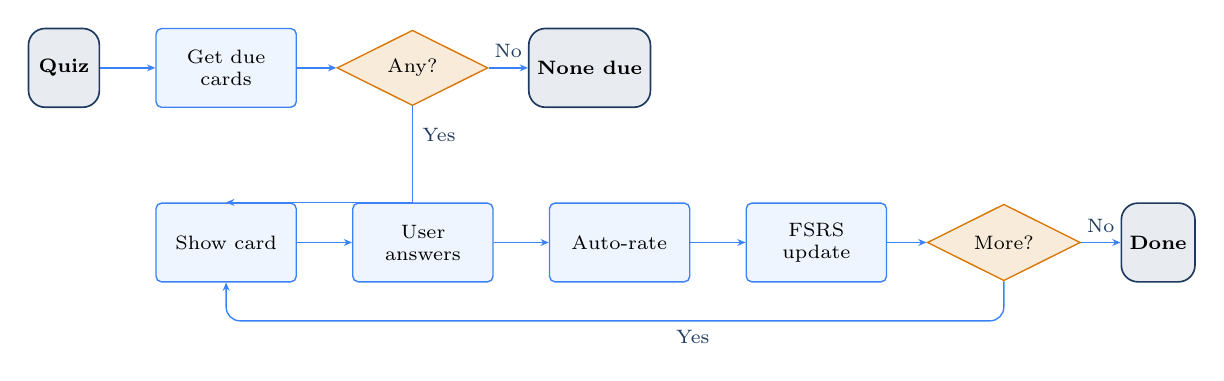
\begin{tikzpicture}[
    node distance=0.7cm and 0.7cm,
    proc/.style={rectangle, rounded corners=2pt, draw=oghmaaccent, fill=oghmaaccent!8,
        minimum height=1cm, text width=1.5cm, align=center, font=\scriptsize,
        line width=0.5pt, inner sep=4pt},
    term/.style={rectangle, rounded corners=6pt, draw=oghmablue, fill=oghmablue!10,
        minimum height=1cm, minimum width=0.9cm, align=center, font=\scriptsize\bfseries,
        line width=0.6pt, inner sep=3pt},
    deci/.style={diamond, draw=decisionamber, fill=decisionamber!15, aspect=2,
        align=center, font=\scriptsize, inner sep=4pt, line width=0.5pt},
    arr/.style={-{Stealth[length=3pt, width=2.5pt]}, line width=0.5pt, oghmaaccent},
    lbl/.style={font=\scriptsize, color=oghmablue}
]
    % row 1: start to first decision
    \node[term] (start) {Quiz};
    \node[proc, right=of start] (fetch) {Get due\\cards};
    \node[deci, right=0.5cm of fetch] (any) {Any?};
    \node[term, right=0.5cm of any] (none) {None due};

    % row 2: main quiz loop
    \node[proc, below=1.2cm of fetch] (show) {Show card};
    \node[proc, right=of show] (answer) {User\\answers};
    \node[proc, right=of answer] (auto) {Auto-rate};
    \node[proc, right=of auto] (update) {FSRS\\update};
    \node[deci, right=0.5cm of update] (more) {More?};
    \node[term, right=0.5cm of more] (summary) {Done};

    % row 1 arrows
    \draw[arr] (start) -- (fetch);
    \draw[arr] (fetch) -- (any);
    \draw[arr] (any) -- node[above, lbl] {No} (none);
    \draw[arr] (any.south) -- node[right, lbl, pos=0.3] {Yes} (any.south |- show.north) -- (show.north);

    % row 2 arrows
    \foreach \a/\b in {show/answer, answer/auto, auto/update}
        \draw[arr] (\a) -- (\b);
    \draw[arr] (update) -- (more);
    \draw[arr] (more) -- node[above, lbl] {No} (summary);

    % loop back: More? --Yes--> Show (route below row 2)
    \draw[arr, rounded corners=5pt] (more.south) -- ++(0,-0.5)
        -| node[below, lbl, pos=0.2] {Yes} (show.south);
\end{tikzpicture}%
}
\caption{Quiz flow: FSRS card scheduling, difficulty rating, and interval update}
\label{fig:quiz-flow}
\end{figure}

\begin{figure}[H]
\centering
\begin{minipage}[t]{0.48\textwidth}
  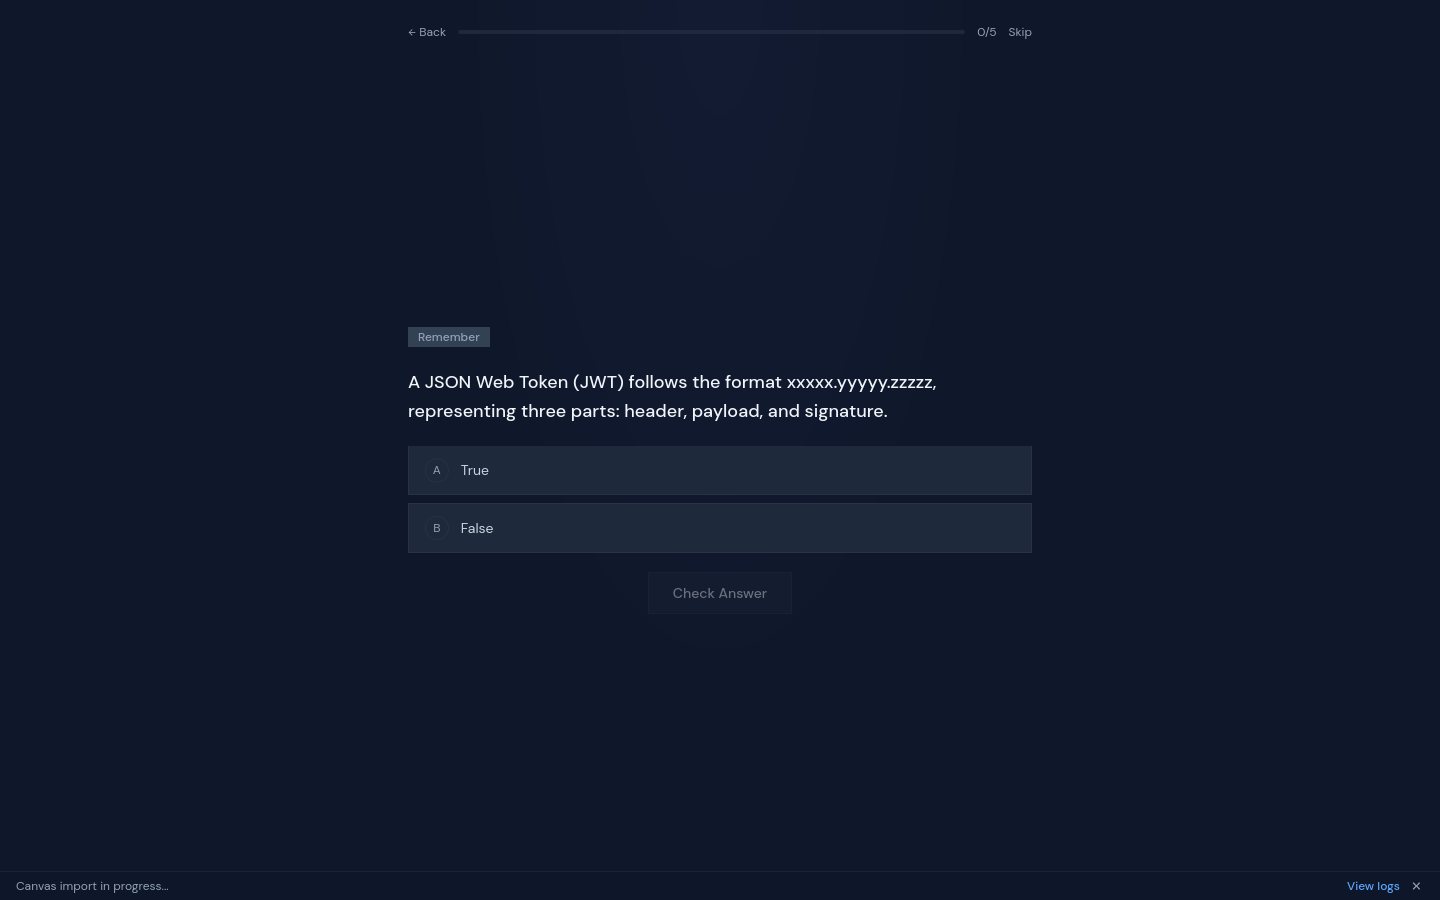
\includegraphics[width=\linewidth]{screenshots/quiz-question}
  \caption*{True/false question generated from CT216 notes}
\end{minipage}\hfill
\begin{minipage}[t]{0.48\textwidth}
  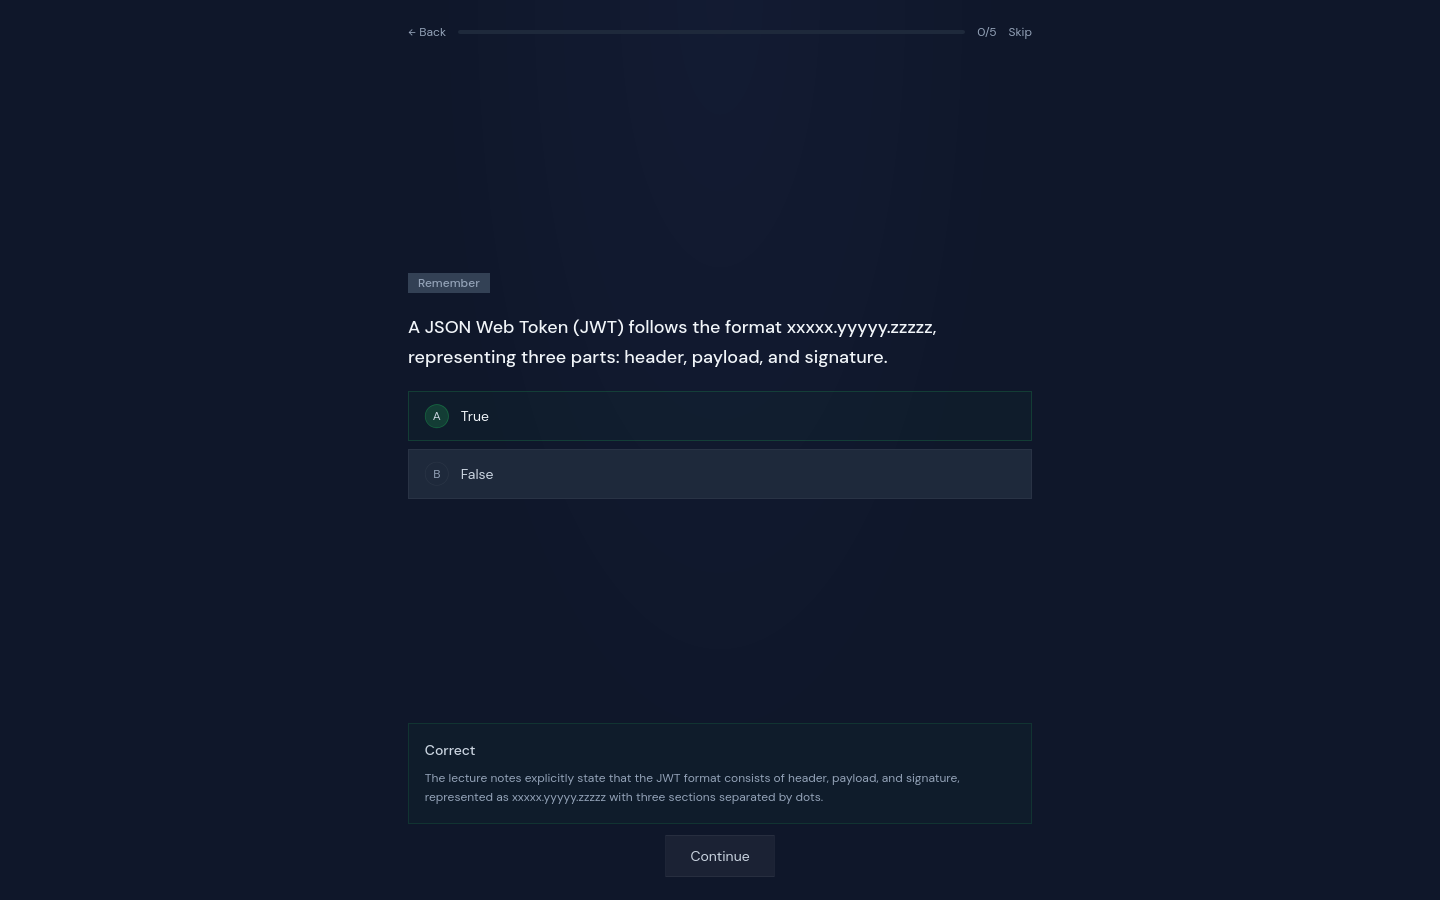
\includegraphics[width=\linewidth]{screenshots/quiz-answer}
  \caption*{Answer revealed with source-grounded explanation}
\end{minipage}
\vspace{0.8em}
\begin{center}
  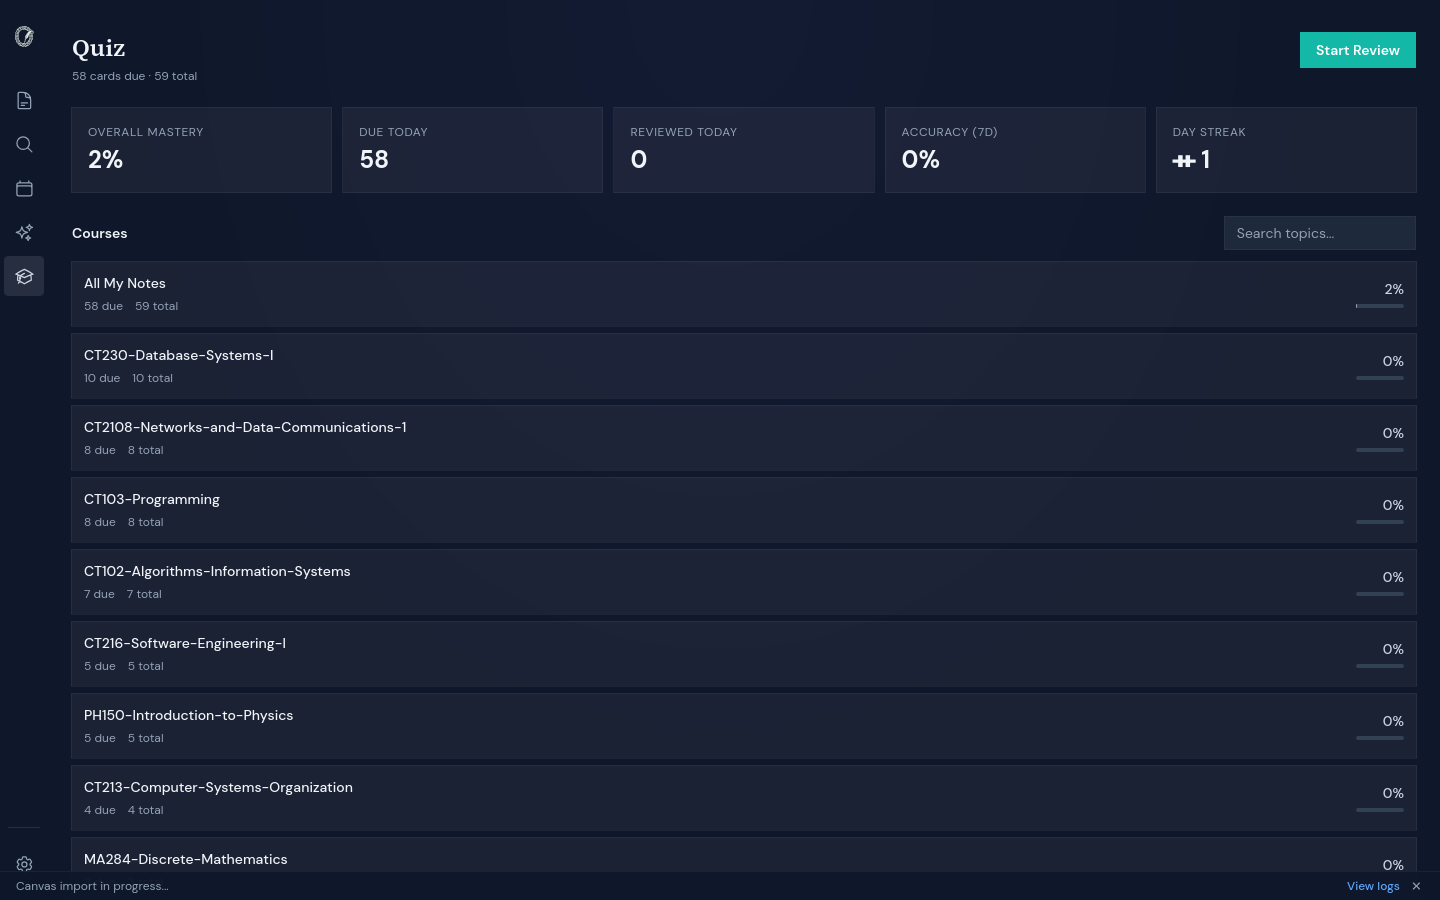
\includegraphics[width=0.72\textwidth]{screenshots/quiz-dashboard}
  \captionof*{figure}{Dashboard: per-course mastery, streak, and due-card counts}
\end{center}
\caption{Quiz system: question view, answer feedback, and course dashboard}
\label{fig:quiz-screenshots}
\end{figure}

\subsection{Productivity Tools}

Additional features include a Pomodoro timer with session tracking, a time-blocking calendar with Canvas assignment display and a subscribable iCal feed (authenticated via a per-user secret token stored in \texttt{app.login.calendar\_export\_token}, allowing direct subscription in any calendar client), and in-viewer PDF annotations.

\screenshot{calendar}{Productivity Tools --- Time-blocking calendar with Canvas assignment integration and iCal subscription}

\subsection{Internationalisation}

OghmaNotes supports 12 languages via a custom locale framework with JSON translation files. The active locale is stored in user preferences and applied across all UI strings.

\screenshot{i18n-language-dropdown}{Language Selector --- All 12 supported locales with flag emojis; Gaeilge (Irish) shown as the active language}

\screenshot{i18n-notes-irish}{Notes Interface in Irish (Gaeilge) --- Navigation, folder tree, and status bar fully localised}


% ══════════════════════════════════════════════════════════════════
% SECTION 5: TECHNICAL ARCHITECTURE
% ══════════════════════════════════════════════════════════════════
\section{Technical Architecture}
\label{sec:architecture}

\subsection{System Overview}

A serverless-first architecture on AWS with three runtime components: Next.js on Amplify, PostgreSQL (RDS with pgvector), and an ECS Fargate import worker, connected via S3, SQS, ElastiCache, and SES (Figure~\ref{fig:architecture}).

\begin{figure}[H]
\centering
\resizebox{\textwidth}{!}{%
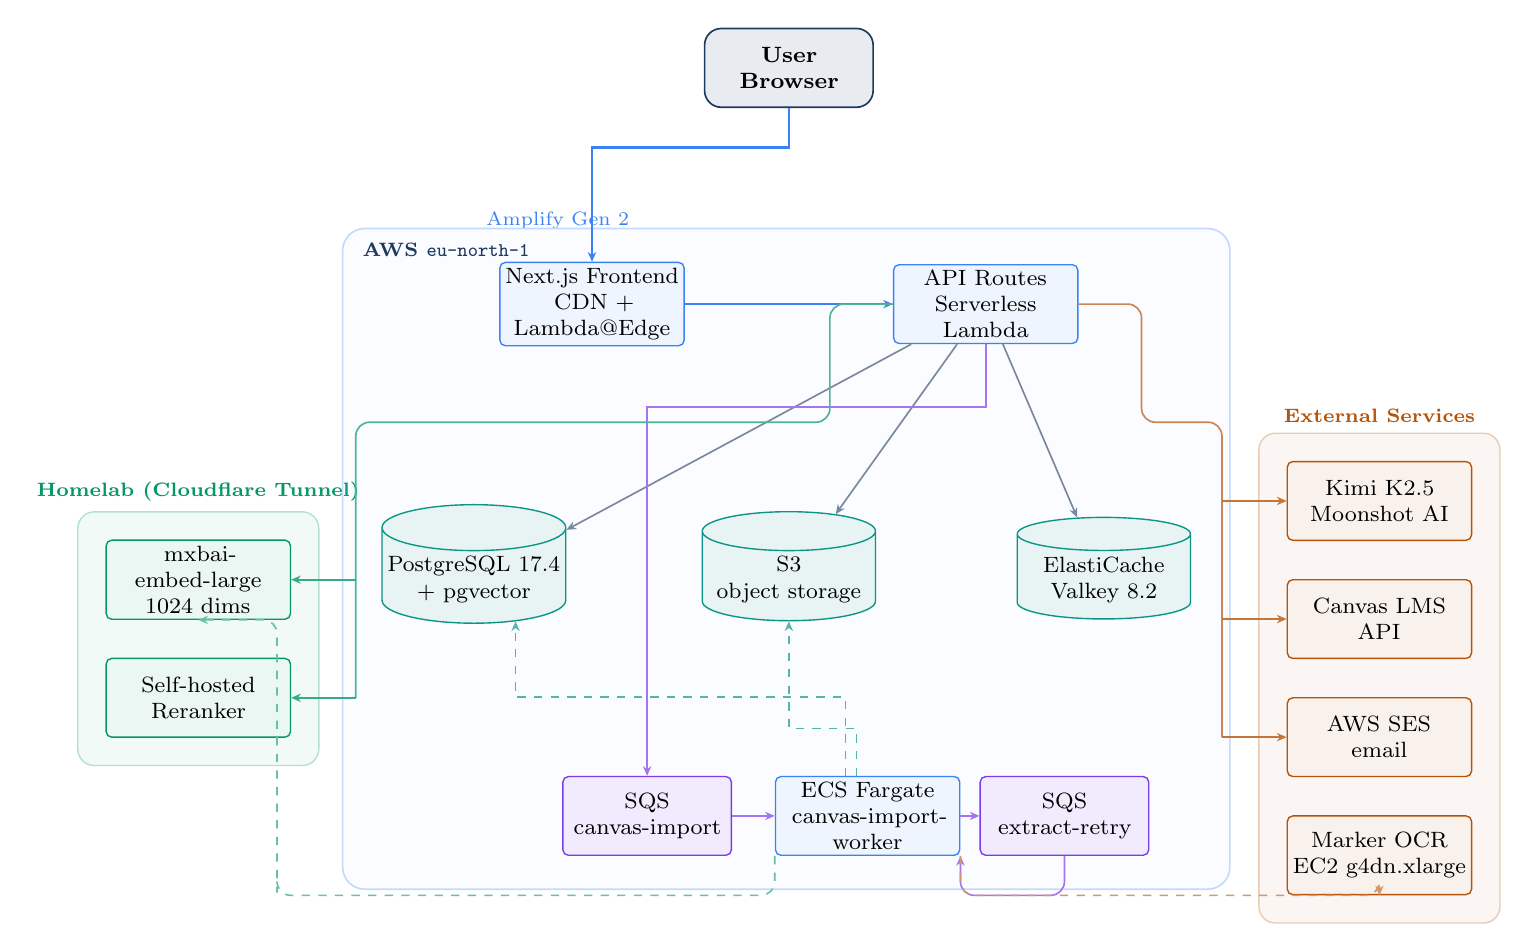
\begin{tikzpicture}[
    % node styles
    comp/.style={rectangle, rounded corners=2pt, draw=oghmaaccent, fill=oghmaaccent!8,
        minimum height=1cm, text width=2.2cm, align=center, font=\footnotesize,
        line width=0.5pt, inner sep=2pt},
    stor/.style={cylinder, draw=storeteal, fill=storeteal!10, shape border rotate=90,
        aspect=0.25, minimum width=2.2cm, minimum height=0.85cm,
        align=center, font=\footnotesize, line width=0.5pt, inner sep=2pt},
    quer/.style={rectangle, rounded corners=2pt, draw=queueviolet, fill=queueviolet!10,
        minimum height=1cm, text width=2cm, align=center, font=\footnotesize,
        line width=0.5pt, inner sep=2pt},
    ext/.style={rectangle, rounded corners=2pt, draw=externalamber, fill=externalamber!8,
        minimum height=1cm, text width=2.2cm, align=center, font=\footnotesize,
        line width=0.5pt, inner sep=2pt},
    home/.style={rectangle, rounded corners=2pt, draw=homelabgreen, fill=homelabgreen!8,
        minimum height=1cm, text width=2.2cm, align=center, font=\footnotesize,
        line width=0.5pt, inner sep=2pt},
    term/.style={rectangle, rounded corners=6pt, draw=oghmablue, fill=oghmablue!10,
        minimum height=1cm, text width=2cm, align=center, font=\footnotesize\bfseries,
        line width=0.6pt, inner sep=2pt},
    arr/.style={-{Stealth[length=3.5pt,width=3pt]}, line width=0.6pt},
    darr/.style={-{Stealth[length=3.5pt,width=3pt]}, line width=0.6pt, dashed}
]
    % === browser ===
    \node[term] (browser) at (0, 0) {User Browser};

    % === AWS: Amplify layer ===
    \node[comp] (fe)  at (-2.5, -3)   {Next.js Frontend\\CDN + Lambda@Edge};
    \node[comp] (api) at ( 2.5, -3)   {API Routes\\Serverless Lambda};

    % === AWS: data stores ===
    \node[stor] (rds)   at (-4,   -6.5) {PostgreSQL 17.4\\+ pgvector};
    \node[stor] (s3)    at ( 0,   -6.5) {S3\\object storage};
    \node[stor] (cache) at ( 4,   -6.5) {ElastiCache\\Valkey 8.2};

    % === AWS: worker layer ===
    \node[quer] (sqs)   at (-1.8, -9.5) {SQS\\canvas-import};
    \node[comp] (ecs)   at ( 1,   -9.5) {ECS Fargate\\canvas-import-worker};
    \node[quer] (retry) at ( 3.5, -9.5) {SQS\\extract-retry};

    % === homelab ===
    \node[home] (embed)  at (-7.5, -6.5) {mxbai-embed-large\\1024 dims};
    \node[home] (rerank) at (-7.5, -8)   {Self-hosted\\Reranker};

    % === external services ===
    \node[ext] (llm)    at (7.5, -5.5)  {Kimi K2.5\\Moonshot AI};
    \node[ext] (canvas) at (7.5, -7)    {Canvas LMS\\API};
    \node[ext] (ses)    at (7.5, -8.5)  {AWS SES\\email};
    \node[ext] (marker) at (7.5, -10)   {Marker OCR\\EC2 g4dn.xlarge};

    % === main request path ===
    % browser -> fe: L-turn
    \draw[arr, color=oghmaaccent, line width=0.8pt]
        (browser.south) -- ++(0,-0.5) -| (fe.north);
    % fe -> api: direct
    \draw[arr, color=oghmaaccent, line width=0.8pt]
        (fe.east) -- (api.west);

    % === API to data stores (direct border-to-border diagonals) ===
    \draw[arr, color=oghmablue!60] (api) -- (rds);
    \draw[arr, color=oghmablue!60] (api) -- (s3);
    \draw[arr, color=oghmablue!60] (api) -- (cache);

    % === API to SQS worker chain ===
    % route: down 0.8, then L-turn left to sqs.north
    \draw[arr, color=queueviolet!70]
        (api.south) -- ++(0,-0.8) -| (sqs.north);
    \draw[arr, color=queueviolet!70] (sqs) -- (ecs);
    \draw[arr, color=queueviolet!70] (ecs) -- (retry);
    \draw[arr, color=queueviolet!70, rounded corners=5pt]
        (retry.south) -- ++(0,-0.5) -| (ecs.south east);

    % === ECS to data stores (dashed) ===
    % offset x slightly so stems don't overlap: s3 branch exits left of centre, rds further left
    \draw[darr, color=storeteal!70]
        ([xshift=-4pt]ecs.north) -- ++(0,0.6) -| (s3.south);
    \draw[darr, color=storeteal!70]
        ([xshift=-8pt]ecs.north) -- ++(0,1) -| (rds.south east);

    % === Homelab bus (left side, x=-5.5 lane) ===
    % entry: api.west -> left 0.8 -> down 1.5 -> sweep left to bus lane -> down to rerank level
    \draw[color=homelabgreen!70, line width=0.6pt, rounded corners=5pt]
        (api.west) -- ++(-0.8,0) -- ++(0,-1.5) -- (-5.5,-4.5) -- (-5.5,-8);
    % branch arrows from bus lane to homelab nodes
    \draw[arr, color=homelabgreen!80] (-5.5,-6.5) -- (embed.east);
    \draw[arr, color=homelabgreen!80] (-5.5,-8)   -- (rerank.east);

    % === ECS to embed (dashed, route via x=-6.5 lane to stay left of bus) ===
    % exit from ecs.south west corner, drop to y=-10.8, go left to x=-6.5, up to embed.south
    \draw[darr, color=homelabgreen!60, rounded corners=5pt]
        (ecs.south west) -- ++(0,-0.5) -| (-6.5,-10.3) |- (embed.south);

    % === External bus (right side, x=5.5 lane) ===
    % entry: api.east -> right 0.8 -> down 1.5 -> sweep right to bus lane -> down to ses level
    \draw[color=externalamber!70, line width=0.6pt, rounded corners=5pt]
        (api.east) -- ++(0.8,0) -- ++(0,-1.5) -- (5.5,-4.5) -- (5.5,-8.5);
    % branch arrows from bus lane to external nodes
    \draw[arr, color=externalamber!80] (5.5,-5.5)  -- (llm.west);
    \draw[arr, color=externalamber!80] (5.5,-7)    -- (canvas.west);
    \draw[arr, color=externalamber!80] (5.5,-8.5)  -- (ses.west);

    % === ECS to Marker (dashed, route below worker row) ===
    % exit from ecs.south east corner to distinguish from ecs->embed exit
    \draw[darr, color=externalamber!60, rounded corners=5pt]
        (ecs.south east) -- ++(0,-0.5) -| (marker.south);

    % === group backgrounds ===
    \begin{scope}[on background layer]
        % Amplify sub-group (drawn first so AWS box encloses it)
        \node[fit=(fe)(api), rounded corners=5pt, fill=oghmaaccent!5,
            draw=oghmaaccent!20, line width=0.4pt, inner sep=8pt,
            label={[font=\scriptsize\color{oghmaaccent},anchor=south west]north west:Amplify Gen 2}] {};
        % AWS outer box (centre column only)
        \node[fit=(fe)(api)(rds)(s3)(cache)(sqs)(ecs)(retry),
            rounded corners=8pt, fill=oghmaaccent!2, draw=oghmaaccent!30,
            line width=0.6pt, inner xsep=14pt, inner ysep=12pt,
            label={[font=\scriptsize\bfseries\color{oghmablue},anchor=north west,xshift=4pt,yshift=-2pt]north west:AWS \texttt{eu-north-1}}] {};
        % Homelab box
        \node[fit=(embed)(rerank), rounded corners=6pt, fill=homelabgreen!5,
            draw=homelabgreen!30, line width=0.5pt, inner sep=10pt,
            label={[font=\scriptsize\bfseries\color{homelabgreen}]north:Homelab (Cloudflare Tunnel)}] {};
        % External box
        \node[fit=(llm)(canvas)(ses)(marker), rounded corners=6pt, fill=externalamber!5,
            draw=externalamber!30, line width=0.5pt, inner sep=10pt,
            label={[font=\scriptsize\bfseries\color{externalamber}]north:External Services}] {};
    \end{scope}
\end{tikzpicture}%
}
\caption{System Architecture --- AWS infrastructure, homelab inference services, and external API dependencies}
\label{fig:architecture}
\end{figure}

\subsection{Technology Stack}

\begin{table}[H]
\centering
\small
\begin{tabularx}{\textwidth}{l>{\raggedright\arraybackslash}X>{\raggedright\arraybackslash}X}
\toprule
\textbf{Layer} & \textbf{Technology} & \textbf{Notes} \\
\midrule
Frontend        & Next.js 16.2, React 19, TypeScript, Tailwind v4 & VSCode-inspired split-pane editor \\
Backend         & Next.js API Routes (serverless)             & REST pattern with route handlers \\
Database        & PostgreSQL 17.4 + pgvector (AWS RDS)        & \tech{app.*} schema, 8+ migrations \\
Object Storage  & AWS S3                                      & Notes, attachments, Canvas files \\
Cache           & AWS ElastiCache (Valkey 8.2)                & Session cache \\
Job Queue       & AWS SQS                                     & Canvas import job dispatch \\
Worker          & AWS ECS Fargate                             & Self-scaling import worker \\
Email           & AWS SES                                     & Password reset, notifications \\
CI/CD           & AWS Amplify Gen 2                           & Build, deploy, CDN, SSR Lambda \\
Auth            & NextAuth v5 + Custom JWT                   & OAuth (Google/GitHub) + AES-256-GCM encryption \\
Embeddings      & \tech{mxbai-embed-large} (homelab, 1024 dims) & Self-hosted via Ollama; see Section~\ref{sec:pivot-8} for migration history \\
Reranking       & \tech{Qwen3-Reranker-4B} (homelab, self-hosted) & Cross-attention reranking for RAG; Cohere deprecated \\
LLM             & Kimi K2.5 (Moonshot AI)                    & Production LLM via OpenAI-compatible API \\
OCR             & Marker (self-hosted EC2 ASG, g4dn.xlarge) + Datalab fallback & PDF/DOCX/PPTX text extraction \\
GPU Compute     & AWS EC2 (g4dn.xlarge, NVIDIA T4, spot \textasciitilde\$0.35/hr) & Marker OCR via ASG, scales to zero \\
LMS             & Canvas LMS REST API                         & Course/file import pipeline \\
i18n            & Custom locale system                        & 12 languages \\
\bottomrule
\end{tabularx}
\caption{OghmaNotes Technology Stack}
\label{tab:tech-stack}
\end{table}

\subsection{AWS Infrastructure}

Production runs in \tech{eu-north-1} (Stockholm). Table~\ref{tab:tech-stack} lists each service. RDS uses a \tech{db.t3.micro} with SSL and all tables under the \tech{app} schema. S3 uses presigned URLs for client-side uploads. SQS decouples the API from the long-running Canvas import worker. ECS Fargate scales to zero when idle. A \tech{g4dn.xlarge} GPU instance (NVIDIA T4, spot pricing) hosts the Marker OCR server behind an Auto Scaling Group that also scales to zero, with the Datalab Convert API as fallback.


% ══════════════════════════════════════════════════════════════════
% SECTION 6: REST API
% ══════════════════════════════════════════════════════════════════
\section{REST API}
\label{sec:api}

The backend exposes 16 REST API route groups under \tech{/api/} via Next.js API Routes, covering authentication, notes CRUD, file operations, Canvas import management, AI chat, search, quiz/flashcard management, productivity features, and data portability.

\subsection{Authentication Middleware}
\label{sec:api-auth}

All protected routes use a custom JWT middleware that extracts the token from HTTP-only cookies, verifies the signature, and attaches the decoded user to the request context. Unauthenticated requests get a 401. Rate limiting uses a sliding-window counter, with tighter limits on auth endpoints (login, register, password reset) to block brute-force attempts.

\begin{table}[H]
\centering
\small
\begin{tabularx}{\textwidth}{lX}
\toprule
\textbf{Route Group} & \textbf{Scope} \\
\midrule
\texttt{/api/auth/*}       & Registration, login, logout, password reset, session \\
\texttt{/api/notes/*}      & Notes CRUD and metadata \\
\texttt{/api/tree}         & Folder hierarchy and drag-and-drop ordering \\
\texttt{/api/upload/*}     & File upload to S3, presigned URL retrieval \\
\texttt{/api/extract}      & PDF text extraction via Marker OCR \\
\texttt{/api/search}       & Combined fuzzy + semantic search \\
\texttt{/api/chat/*}       & RAG chat and session management \\
\texttt{/api/canvas/*}     & Canvas connection, course listing, import, status \\
\texttt{/api/quiz/*}       & Quiz sessions, answers, flashcards, streaks, dashboard \\
\texttt{/api/pomodoro}     & Pomodoro timer sessions \\
\texttt{/api/time-blocks}  & Time block calendar management \\
\texttt{/api/settings}     & User preferences and account management \\
\texttt{/api/annotations}  & PDF annotation storage \\
\texttt{/api/calendar}     & iCal feed export (per-user secret token) \\
\texttt{/api/export}       & Vault ZIP export \\
\texttt{/api/embeddings}   & Embedding pipeline status and ingestion management \\
\bottomrule
\end{tabularx}
\caption{REST API Route Groups (16 total)}
\label{tab:api-routes}
\end{table}


% ══════════════════════════════════════════════════════════════════
% SECTION 7: KEY SYSTEM FLOWS
% ══════════════════════════════════════════════════════════════════
\section{Key System Flows}
\label{sec:flows}

\subsection{Authentication Flow}
\label{sec:flow-auth}

Three paths converge on a shared JWT session: email/password login (bcrypt), registration (SES email verification), and OAuth via Google/GitHub (Auth.js). All paths issue an HTTP-only JWT cookie encrypted with AES-256-GCM. Token refresh goes through \tech{/api/auth/me}.

\begin{figure}[H]
\centering
\resizebox{\textwidth}{!}{%
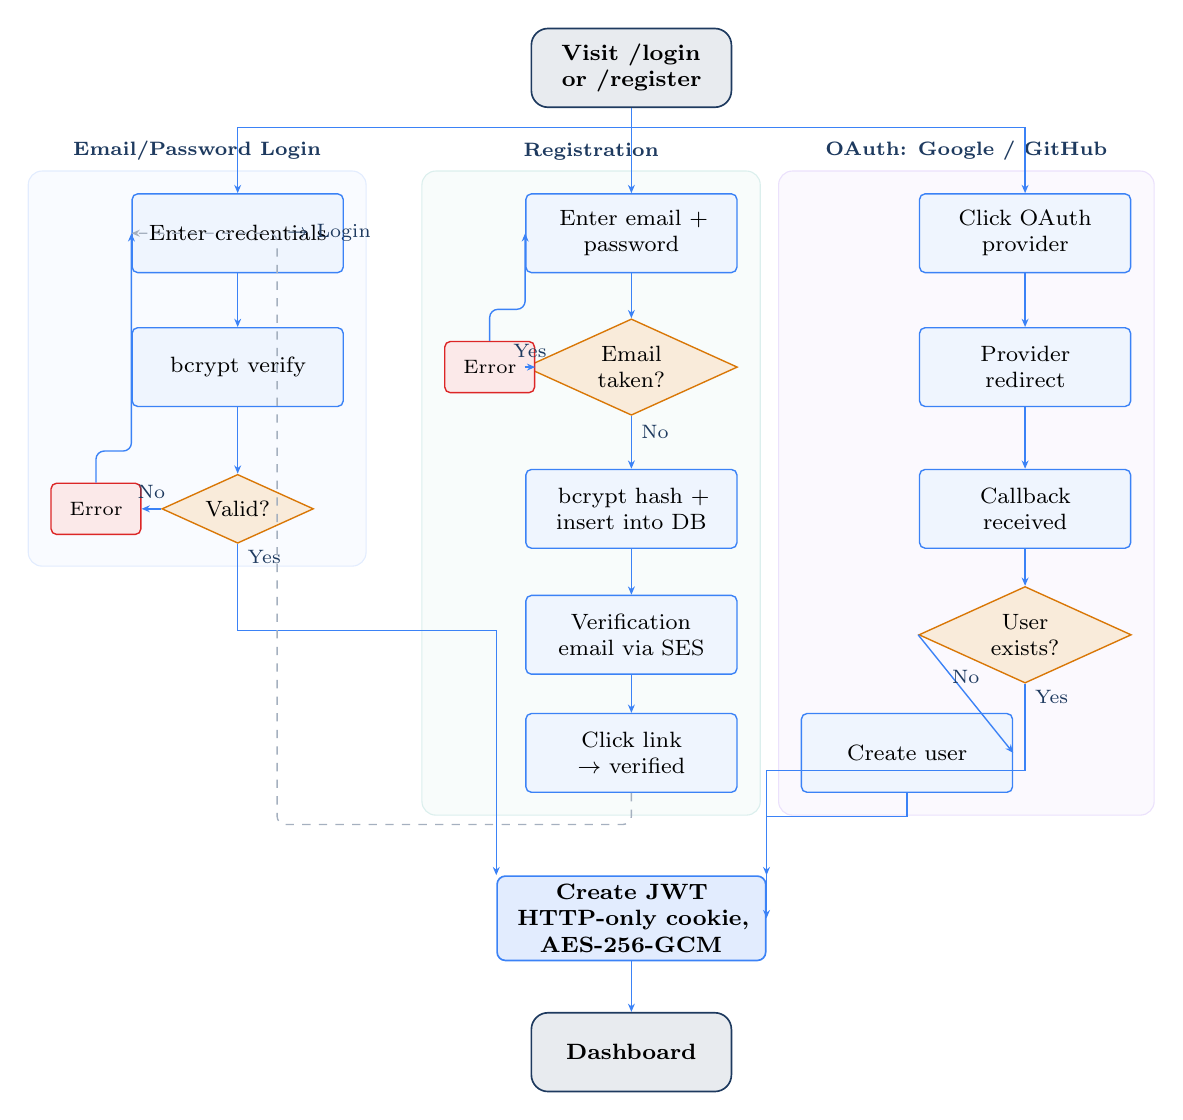
\begin{tikzpicture}[
    proc/.style={rectangle, rounded corners=2pt, draw=oghmaaccent, fill=oghmaaccent!8,
        minimum height=1cm, text width=2.4cm, align=center, font=\footnotesize,
        line width=0.5pt, inner sep=4pt},
    term/.style={rectangle, rounded corners=6pt, draw=oghmablue, fill=oghmablue!10,
        minimum height=1cm, text width=2.4cm, align=center, font=\footnotesize\bfseries,
        line width=0.6pt, inner sep=2pt},
    deci/.style={diamond, draw=decisionamber, fill=decisionamber!15, aspect=2.2,
        align=center, font=\footnotesize, inner sep=3pt, line width=0.5pt},
    err/.style={rectangle, rounded corners=2pt, draw=errorred, fill=errorred!10,
        minimum height=0.65cm, text width=1cm, align=center, font=\scriptsize,
        line width=0.5pt, inner sep=2pt},
    jwt/.style={rectangle, rounded corners=3pt, draw=oghmaaccent, fill=oghmaaccent!15,
        minimum height=0.85cm, text width=3.2cm, align=center, font=\footnotesize\bfseries,
        line width=0.6pt, inner sep=3pt},
    arr/.style={-{Stealth[length=3pt, width=2.5pt]}, line width=0.5pt, oghmaaccent},
    lbl/.style={font=\scriptsize, color=oghmablue}
]
    % === start ===
    \node[term] (start) at (0, 0) {Visit /login or /register};

    % === column 1: email/password login (left) ===
    \node[proc] (l1) at (-5, -2.1) {Enter credentials};
    \node[proc] (l2) at (-5, -3.8) {bcrypt verify};
    \node[deci] (l3) at (-5, -5.6) {Valid?};
    \node[err]  (l4) at (-6.8, -5.6) {Error};

    % === column 2: registration (centre) ===
    \node[proc] (r1) at (0, -2.1) {Enter email +\\password};
    \node[deci] (r2) at (0, -3.8) {Email\\taken?};
    \node[err]  (r3) at (-1.8, -3.8) {Error};
    \node[proc] (r4) at (0, -5.6) {bcrypt hash +\\insert into DB};
    \node[proc] (r5) at (0, -7.2) {Verification\\email via SES};
    \node[proc] (r6) at (0, -8.7) {Click link\\$\to$ verified};

    % === column 3: OAuth (right) ===
    \node[proc] (o1) at (5, -2.1) {Click OAuth\\provider};
    \node[proc] (o2) at (5, -3.8) {Provider\\redirect};
    \node[proc] (o3) at (5, -5.6) {Callback\\received};
    \node[deci] (o4) at (5, -7.2) {User\\exists?};
    \node[proc] (o5) at (3.5, -8.7) {Create user};

    % === convergence ===
    \node[jwt] (jwt) at (0, -10.8) {Create JWT\\HTTP-only cookie, AES-256-GCM};
    \node[term] (dash) at (0, -12.5) {Dashboard};

    % --- arrows from start ---
    \draw[arr] (start.south) -- ++(0,-0.25) -| (l1.north);
    \draw[arr] (start.south) -- (r1.north);
    \draw[arr] (start.south) -- ++(0,-0.25) -| (o1.north);

    % --- login flow ---
    \draw[arr] (l1) -- (l2);
    \draw[arr] (l2) -- (l3);
    \draw[arr] (l3) -- node[above, lbl] {No} (l4);
    \draw[arr, rounded corners=3pt] (l4.north) -- ++(0,0.4) -| (l1.west);
    \draw[arr] (l3.south) -- node[right, lbl, pos=0.15] {Yes} ++(0,-1.1) -| (jwt.north west);

    % --- registration flow ---
    \draw[arr] (r1) -- (r2);
    \draw[arr] (r2) -- node[above, lbl] {Yes} (r3);
    \draw[arr, rounded corners=3pt] (r3.north) -- ++(0,0.4) -| (r1.west);
    \draw[arr] (r2.south) -- node[right, lbl, pos=0.3] {No} (r4);
    \draw[arr] (r4) -- (r5);
    \draw[arr] (r5) -- (r6);
    \draw[arr, draw=oghmablue!40, dashed, rounded corners=3pt]
        (r6.south) -- ++(0,-0.4) -- ++(-4.5,0)
        |- node[right, lbl, pos=0.50] {$\to$ Login} (l1.west);

    % --- OAuth flow ---
    \draw[arr] (o1) -- (o2);
    \draw[arr] (o2) -- (o3);
    \draw[arr] (o3) -- (o4);
    \draw[arr] (o4.west) -- node[above, lbl] {No} (o5.east);
    \draw[arr] (o5.south) -- ++(0,-0.3) -| (jwt.east);
    \draw[arr] (o4.south) -- node[right, lbl, pos=0.15] {Yes} ++(0,-1.1) -| (jwt.north east);

    % --- JWT to dashboard ---
    \draw[arr] (jwt) -- (dash);

    % --- group backgrounds ---
    \begin{scope}[on background layer]
        \node[fit=(l1)(l2)(l3)(l4), rounded corners=5pt, fill=oghmaaccent!3,
            draw=oghmaaccent!15, line width=0.4pt, inner sep=8pt,
            label={[font=\scriptsize\bfseries\color{oghmablue}]north:Email/Password Login}] {};
        \node[fit=(r1)(r2)(r3)(r4)(r5)(r6), rounded corners=5pt, fill=storeteal!3,
            draw=storeteal!15, line width=0.4pt, inner sep=8pt,
            label={[font=\scriptsize\bfseries\color{oghmablue}]north:Registration}] {};
        \node[fit=(o1)(o2)(o3)(o4)(o5), rounded corners=5pt, fill=queueviolet!3,
            draw=queueviolet!15, line width=0.4pt, inner sep=8pt,
            label={[font=\scriptsize\bfseries\color{oghmablue}]north:OAuth: Google / GitHub}] {};
    \end{scope}
\end{tikzpicture}%
}
\caption{Authentication Flow --- Email/password, registration with email verification, and OAuth paths}
\label{fig:auth-flow}
\end{figure}

\subsection{Canvas Import Pipeline}
\label{sec:flow-canvas}

The Canvas import touches five AWS services. The API creates a job record and publishes to SQS. An ECS Fargate worker picks it up and runs: Canvas API file retrieval $\to$ S3 upload $\to$ Marker OCR text extraction (Datalab fallback) $\to$ sentence-aligned chunking ($\sim$500 chars) $\to$ embedding via self-hosted model $\to$ pgvector storage. The worker scales to zero after an idle timeout.

\begin{figure}[H]
\centering
\resizebox{\textwidth}{!}{%
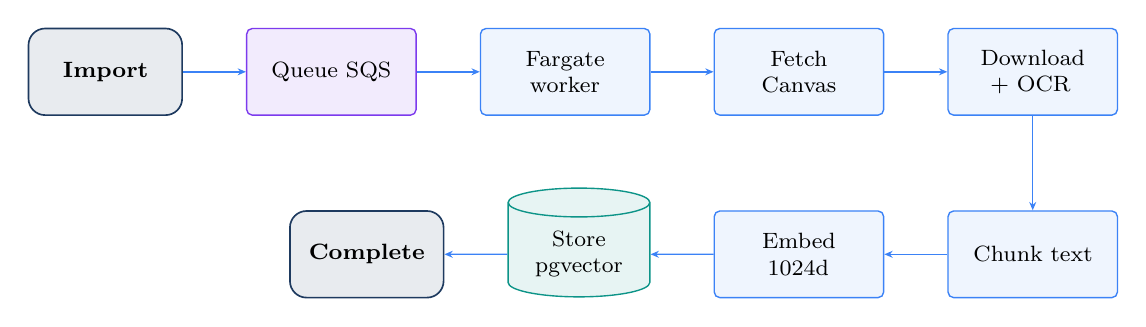
\begin{tikzpicture}[
    node distance=0.8cm and 0.8cm,
    proc/.style={rectangle, rounded corners=2pt, draw=oghmaaccent, fill=oghmaaccent!8,
        minimum height=1.1cm, text width=1.8cm, align=center, font=\footnotesize,
        line width=0.5pt, inner sep=5pt},
    term/.style={rectangle, rounded corners=6pt, draw=oghmablue, fill=oghmablue!10,
        minimum height=1.1cm, text width=1.6cm, align=center, font=\footnotesize\bfseries,
        line width=0.6pt, inner sep=5pt},
    stor/.style={cylinder, draw=storeteal, fill=storeteal!10, shape border rotate=90,
        aspect=0.25, minimum width=1.8cm, minimum height=1.1cm,
        align=center, font=\footnotesize, line width=0.5pt, inner sep=5pt},
    quer/.style={rectangle, rounded corners=2pt, draw=queueviolet, fill=queueviolet!10,
        minimum height=1.1cm, text width=1.8cm, align=center, font=\footnotesize,
        line width=0.5pt, inner sep=5pt},
    arr/.style={-{Stealth[length=3pt, width=2.5pt]}, line width=0.5pt, oghmaaccent}
]
    % top row: left to right
    \node[term] (u) {Import};
    \node[quer, right=of u] (q) {Queue SQS};
    \node[proc, right=of q] (w) {Fargate\\worker};
    \node[proc, right=of w] (f) {Fetch\\Canvas};
    \node[proc, right=of f] (d) {Download\\+ OCR};

    % bottom row: right to left
    \node[proc, below=1.2cm of d] (c) {Chunk text};
    \node[proc, left=of c] (e) {Embed\\1024d};
    \node[stor, left=of e] (s) {Store\\pgvector};
    \node[term, left=of s] (done) {Complete};

    % top row arrows
    \foreach \a/\b in {u/q, q/w, w/f, f/d}
        \draw[arr] (\a) -- (\b);
    % turn
    \draw[arr] (d) -- (c);
    % bottom row arrows
    \foreach \a/\b in {c/e, e/s, s/done}
        \draw[arr] (\a) -- (\b);
\end{tikzpicture}%
}
\caption{Canvas Import Pipeline --- SQS job dispatch, ECS Fargate worker processing, and pgvector storage}
\label{fig:canvas-pipeline}
\end{figure}

\subsection{RAG Query Flow}
\label{sec:flow-rag}

The query is embedded (self-hosted \tech{mxbai-embed-large}, 1024d), searched against stored chunks via pgvector cosine similarity (top-20 within distance 0.75, optionally scoped to selected files), reranked by a self-hosted cross-attention model (top-5 above a 0.15 relevance floor), injected into a prompt, and streamed to the user from Kimi K2.5 via SSE. Messages and responses are persisted for session continuity. Thresholds were tuned empirically against university lecture queries.

\begin{figure}[H]
\centering
\resizebox{\textwidth}{!}{%
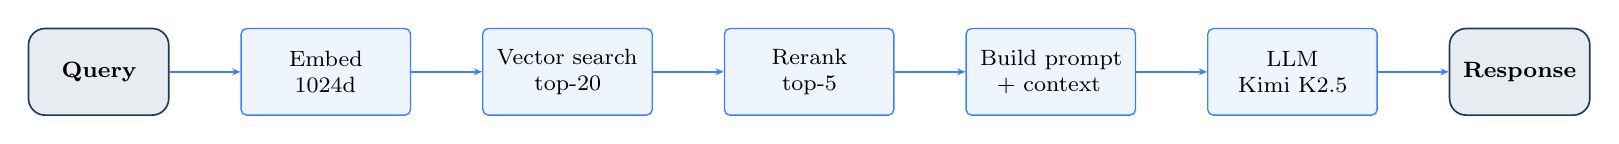
\begin{tikzpicture}[
    node distance=0.9cm,
    proc/.style={rectangle, rounded corners=2pt, draw=oghmaaccent, fill=oghmaaccent!8,
        minimum height=1.1cm, text width=1.8cm, align=center, font=\footnotesize,
        line width=0.5pt, inner sep=5pt},
    term/.style={rectangle, rounded corners=6pt, draw=oghmablue, fill=oghmablue!10,
        minimum height=1.1cm, text width=1.5cm, align=center, font=\footnotesize\bfseries,
        line width=0.6pt, inner sep=4pt},
    arr/.style={-{Stealth[length=3pt, width=2.5pt]}, line width=0.5pt, oghmaaccent}
]
    \node[term] (q) {Query};
    \node[proc, right=of q] (e) {Embed\\1024d};
    \node[proc, right=of e] (s) {Vector search\\top-20};
    \node[proc, right=of s] (r) {Rerank\\top-5};
    \node[proc, right=of r] (p) {Build prompt\\+ context};
    \node[proc, right=of p] (l) {LLM\\Kimi K2.5};
    \node[term, right=of l] (o) {Response};

    \foreach \a/\b in {q/e, e/s, s/r, r/p, p/l, l/o}
        \draw[arr] (\a) -- (\b);
\end{tikzpicture}%
}
\caption{RAG Query Pipeline --- Query embedding, pgvector cosine search, self-hosted reranking, and LLM streaming}
\label{fig:rag-flow}
\end{figure}


% ══════════════════════════════════════════════════════════════════
% SECTION 8: DATABASE DESIGN
% ══════════════════════════════════════════════════════════════════
\section{Database Design}
\label{sec:database}

\subsection{Schema Overview}

\begin{sloppypar}
PostgreSQL~17.4 with \tech{pgvector}, hosted on AWS RDS. All 19 tables sit under the \tech{app} schema. Core tables: \tech{app.login} (users), \tech{app.notes}/\tech{app.tree\_items} (content and file hierarchy), \tech{app.chunks}/\tech{app.embeddings} (RAG vectors), and \tech{app.chat\_sessions}/\tech{app.chat\_messages} (conversations). Supporting tables cover OAuth linking, Canvas imports, quiz flashcards, Pomodoro sessions, time blocks, PDF annotations, and rate limiting. The schema went through 23 tracked versions in \tech{app.schema\_migrations}, covering the embedding dimension change (Section~\ref{sec:pivot-8}), two-phase Canvas import, rate limit audit logging, quiz infrastructure, chat message rating, and per-user calendar export tokens.
\end{sloppypar}

\screenshotplaceholder{Entity-Relationship Diagram --- Database schema relationships}

\subsection{Vector Storage}

Each chunk's 1024-dimensional embedding is stored via pgvector with HNSW indexing for approximate nearest-neighbour search. The embedding column was migrated from \tech{vector(4096)} to \tech{vector(1024)} as part of Section~\ref{sec:pivot-8}, with all content re-embedded (see Section~\ref{sec:pivots}).


% ══════════════════════════════════════════════════════════════════
% SECTION 9: CI/CD & DEPLOYMENT
% ══════════════════════════════════════════════════════════════════
\section{CI/CD \& Deployment}
\label{sec:cicd}

\subsection{AWS Amplify Pipeline}

The project uses AWS Amplify Gen~2 for CI/CD. Every push to \tech{main} triggers the pipeline, which runs through three stages:

\begin{enumerate}[leftmargin=1.5em]
    \item \textbf{Install:} Runs \tech{npm ci} to install dependencies from the lockfile.
    \item \textbf{Build:} Executes \tech{next build}, producing optimised static assets and serverless functions.
    \item \textbf{Deploy:} Distributes the build output to Amplify's CDN and deploys SSR routes as Lambda@Edge functions.
\end{enumerate}

Environment variables (database credentials, API keys, AWS service endpoints) are managed through Amplify's environment configuration, with separate sets for the \tech{dev} and \tech{main} branches.

\subsection{Branch Strategy}

The repository uses two branches. \tech{dev} is where features are built and tested. When stable, they merge to \tech{main} via pull request, which triggers the production deployment. Each branch has its own Amplify environment with an independent configuration.

\subsection{Containerised Infrastructure}

\begin{sloppypar}
The repository has three Dockerfiles, each for a distinct runtime: the Next.js production app (three-stage Alpine build with standalone output), the Canvas import worker (\tech{Dockerfile.worker}, Node 22 with \tech{tsx}), and the Marker OCR service (\tech{Dockerfile.marker}, Python 3.11 with GPU support). Worker and Marker images are pushed to Amazon ECR. ECS Fargate pulls the worker image on demand, scaling from zero when SQS messages arrive.

A Husky~v9 pre-commit hook enforces quality gates on every commit: full ESLint linting and the Vitest test suite (blocking), \tech{Dockerfile.marker} syntax validation via \tech{docker build --dry-run}, and \tech{shellcheck} on infrastructure shell scripts. For the Marker OCR instance, a custom AMI baking script (\tech{bake-ami.sh}) pre-installs Python dependencies and the CUDA runtime into a machine image, cutting cold-start time from 5--7~minutes to around 90~seconds. The baked AMI is deployed via a Launch Template inside an Auto Scaling Group behind an Application Load Balancer, with IAM roles granting ECR pull access.
\end{sloppypar}

\begin{figure}[H]
\centering
\resizebox{\textwidth}{!}{%
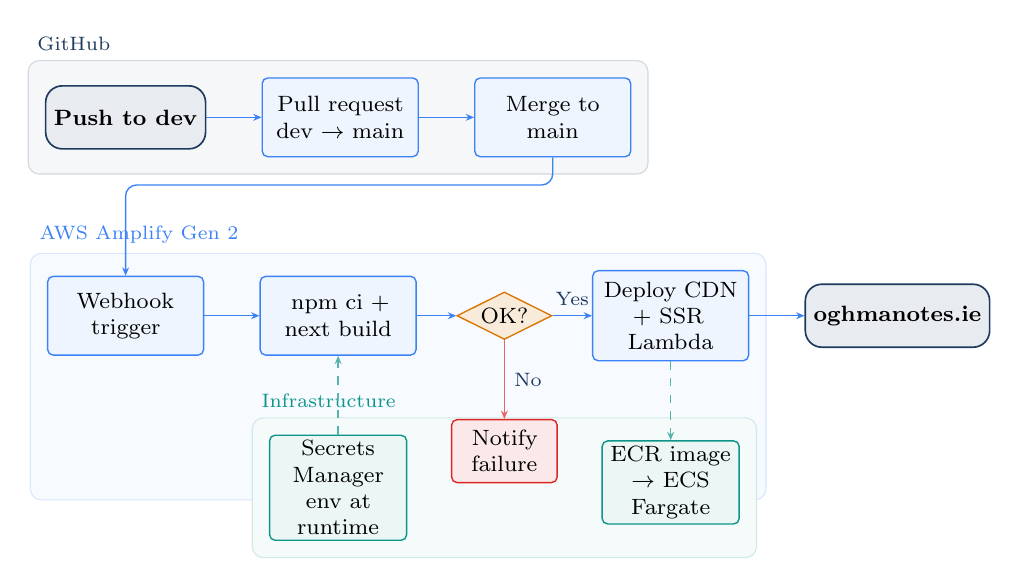
\begin{tikzpicture}[
    node distance=0.7cm and 0.7cm,
    proc/.style={rectangle, rounded corners=2pt, draw=oghmaaccent, fill=oghmaaccent!8,
        minimum height=1cm, text width=1.7cm, align=center, font=\footnotesize,
        line width=0.5pt, inner sep=4pt},
    term/.style={rectangle, rounded corners=6pt, draw=oghmablue, fill=oghmablue!10,
        minimum height=0.8cm, minimum width=1.2cm, align=center, font=\footnotesize\bfseries,
        line width=0.6pt, inner sep=3pt},
    deci/.style={diamond, draw=decisionamber, fill=decisionamber!15, aspect=2,
        align=center, font=\footnotesize, inner sep=1pt, line width=0.5pt},
    fail/.style={rectangle, rounded corners=2pt, draw=errorred, fill=errorred!10,
        minimum height=0.8cm, text width=1.2cm, align=center, font=\footnotesize,
        line width=0.5pt, inner sep=2pt},
    infra/.style={rectangle, rounded corners=2pt, draw=storeteal, fill=storeteal!8,
        minimum height=0.8cm, text width=1.6cm, align=center, font=\footnotesize,
        line width=0.5pt, inner sep=2pt},
    arr/.style={-{Stealth[length=3pt, width=2.5pt]}, line width=0.5pt, oghmaaccent},
    lbl/.style={font=\scriptsize, color=oghmablue}
]
    % row 1: GitHub flow
    \node[term] (dev) {Push to dev};
    \node[proc, right=of dev] (pr) {Pull request\\dev $\to$ main};
    \node[proc, right=of pr] (merge) {Merge to\\main};

    % row 2: Amplify build + deploy
    \node[proc, below=1.6cm of dev] (hook) {Webhook\\trigger};
    \node[proc, right=of hook] (build) {npm ci +\\next build};
    \node[deci, right=0.5cm of build] (check) {OK?};
    \node[proc, right=0.5cm of check] (deploy) {Deploy CDN\\+ SSR Lambda};
    \node[term, right=of deploy] (live) {oghmanotes.ie};

    % fail branch
    \node[fail, below=1cm of check] (fail) {Notify\\failure};

    % infra row
    \node[infra, below=1cm of build] (secrets) {Secrets Manager\\env at runtime};
    \node[infra, below=1cm of deploy] (ecr) {ECR image\\$\to$ ECS Fargate};

    % row 1 arrows
    \foreach \a/\b in {dev/pr, pr/merge}
        \draw[arr] (\a) -- (\b);
    % connect rows
    \draw[arr, rounded corners=4pt] (merge.south) -- ++(0,-0.35) -| (hook.north);
    % row 2 arrows
    \draw[arr] (hook) -- (build);
    \draw[arr] (build) -- (check);
    \draw[arr] (check) -- node[above, lbl] {Yes} (deploy);
    \draw[arr] (deploy) -- (live);

    % fail
    \draw[arr, draw=errorred!70] (check.south) -- node[right, lbl] {No} (fail);

    % infra connections
    \draw[arr, draw=storeteal!70, dashed] (secrets) -- (build);
    \draw[arr, draw=storeteal!70, dashed] (deploy) -- (ecr);

    % group backgrounds
    \begin{scope}[on background layer]
        \node[fit=(dev)(pr)(merge), rounded corners=4pt, fill=oghmablue!4,
            draw=oghmablue!20, line width=0.4pt, inner sep=6pt,
            label={[font=\scriptsize\color{oghmablue}, anchor=south west]north west:GitHub}] {};
        \node[fit=(hook)(build)(check)(deploy)(fail), rounded corners=4pt, fill=oghmaaccent!4,
            draw=oghmaaccent!20, line width=0.4pt, inner sep=6pt,
            label={[font=\scriptsize\color{oghmaaccent}, anchor=south west]north west:AWS Amplify Gen 2}] {};
        \node[fit=(secrets)(ecr), rounded corners=4pt, fill=storeteal!4,
            draw=storeteal!20, line width=0.4pt, inner sep=6pt,
            label={[font=\scriptsize\color{storeteal}, anchor=south west]north west:Infrastructure}] {};
    \end{scope}
\end{tikzpicture}%
}
\caption{CI/CD Pipeline --- GitHub push to AWS Amplify build, deploy, and infrastructure update}
\label{fig:cicd}
\end{figure}


% ══════════════════════════════════════════════════════════════════
% SECTION 10: DESIGN DECISIONS & ARCHITECTURAL PIVOTS
% ══════════════════════════════════════════════════════════════════
\section{Design Decisions \& Architectural Pivots}
\label{sec:pivots}

The team made several architectural pivots during development, each driven by constraints hit at runtime.

\subsection{Pivot 1: Notea Fork to Modern Next.js Application}
\label{sec:pivot-1}

The project started from Notea, an MIT-licensed, unmaintained note-taking app that stored markdown on S3, a useful backbone to scaffold from. Notea's codebase ran on outdated dependencies throughout the stack. Modernising it meant upgrading through three major React versions (16~$\to$~19), where APIs were deprecated or removed, replacing the legacy editor with Lexical and CodeMirror, and swapping unmaintained packages for supported alternatives. That upgrade work was heavy, but it left the team with a production-ready S3-backed markdown foundation to build RAG, Canvas integration, and the full AWS infrastructure on top of.

In hindsight, forking saved early scaffolding time but the unmaintained dependency tree created upgrade debt that compounded with every major framework version.

\subsection{Pivot 2: Monorepo to Single Application}
\label{sec:pivot-2}

The project started as a monorepo with separate packages under an \tech{apps/web/} directory. The added complexity in Amplify's build configuration wasn't worth it for a three-person team. Collapsing to a single Next.js application simplified both development and deployment.

\subsection{Pivot 3: BullMQ (Redis) to AWS SQS}
\label{sec:pivot-3}

The Canvas import job queue started as BullMQ backed by ElastiCache (Valkey/Redis). It worked locally but broke in production: Amplify's Lambda functions couldn't reach ElastiCache without VPC configuration, and the Lambda runtime's 29-second timeout was incompatible with long-running import jobs. Migrating to AWS SQS fixed both problems. SQS uses IAM authentication (no VPC needed) and fully decouples the API from the worker.

Cloud networking constraints ended up shaping the architecture more than any theoretical best practice would have.

\subsection{Pivot 4: Local Ollama to Cohere Embeddings}
\label{sec:pivot-4}

\begin{sloppypar}
The initial embedding pipeline used a self-hosted Ollama instance running \tech{qwen3-embedding:8b}, served over a Cloudflare Tunnel. The model was fine. The tunnel was not. Embedding requests during Canvas imports would intermittently time out, causing ingestion jobs to fail mid-batch. Rather than debug the tunnel, the team migrated to Cohere's \tech{embed-multilingual-v3.0} API, which gave a stable endpoint with consistent latency. Cohere's 1024-dimensional output was also compatible with pgvector's HNSW index limit.
\end{sloppypar}

Infrastructure reliability turned out to matter as much as model quality --- a tunnelled connection introduces failure modes that a direct API call simply does not have.

\subsection{Pivot 5: OpenWebUI as Secure Model Gateway}
\label{sec:pivot-5}

The homelab models (embedding, reranking) sit behind OpenWebUI, which handles auth and exposes them over a Cloudflare Tunnel with sign-ups disabled. Kimi K2.5 is called directly via its OpenAI-compatible API. Switching between self-hosted and cloud providers is a single environment variable change.

\subsection{Pivot 6: pnpm to npm}
\label{sec:pivot-6}

A mid-project switch from pnpm to npm was forced by compatibility issues with the Amplify build environment. pnpm's workspace features conflicted with Amplify's build process. Switching to npm resolved the build failures with minimal disruption.

\subsection{Pivot 7: Cohere Embeddings Back to Self-Hosted Homelab}
\label{sec:pivot-7}

After migrating to Cohere (Section~\ref{sec:pivot-4}), the team hit aggressive rate limiting on Cohere's free-tier embedding API during Canvas imports, where hundreds of chunks needed embedding in quick succession. Rather than pay for a higher tier, the team fixed the underlying Cloudflare Tunnel reliability issues and moved back to the self-hosted \tech{qwen3-embedding:8b} model on the project lead's homelab. That eliminated rate limits and external API costs. With the tunnel stable, the team also restored the original 4096-dimensional vectors for better semantic fidelity, accepting sequential pgvector scanning at current data scale. The reranker moved to self-hosted infrastructure at the same time.

External APIs introduce constraints beyond just cost --- rate limits can silently degrade the user experience in ways that are hard to debug, and self-hosting trades that unpredictability for operational responsibility.

\subsection{Pivot 8: qwen3-embedding:8b to mxbai-embed-large (Right-Sizing for Hardware)}
\label{sec:pivot-8}

After restoring self-hosted embeddings (Section~\ref{sec:pivot-7}), the team hit a hardware bottleneck. The \tech{qwen3-embedding:8b} model needed 6.1\,GB of memory, but the server's GPU (a GTX~1050~Ti Max-Q) had only 4\,GB of VRAM. Ollama split the model automatically: 59\% on GPU, 41\% falling back to CPU on the i7-8750H. That CPU portion became the dominant bottleneck, causing erratic latency that varied with whatever else the CPU was doing.

Running it entirely on CPU would have been worse. Instead, the team switched to \tech{mxbai-embed-large}, a 335M-parameter model that fits within the 4\,GB VRAM budget. The migration required changing the schema from \tech{vector(4096)} to \tech{vector(1024)}, clearing all existing embeddings, and re-embedding everything. A secondary benefit: 1024~dimensions falls within pgvector's HNSW index limit of 2000, enabling approximate nearest-neighbour indexing that wasn't possible at 4096 dimensions.

A smaller model running entirely on GPU will consistently beat a larger one partially offloaded to CPU --- benchmark quality means nothing if the inference environment can't support it. Right-sizing to the available hardware eliminated the erratic latency and improved embedding throughput by roughly 10$\times$.

\subsection{Budget Constraints}
\label{sec:budget}

The project ran on AWS education credits. That budget directly shaped infrastructure decisions: the self-scaling ECS Fargate pattern (scaling to zero when idle) was chosen to keep compute costs low. Instance sizes were kept minimal (\tech{db.t3.micro} for RDS, \tech{cache.t3.micro} for ElastiCache), and everything was deployed to a single region (\tech{eu-north-1}) to avoid cross-region transfer costs.


% ══════════════════════════════════════════════════════════════════
% SECTION 11: TESTING
% ══════════════════════════════════════════════════════════════════
\section{Testing}
\label{sec:testing}

The project uses Vitest as its test framework. The test suite comprises 52 test files covering: authentication (JWT, bcrypt, OAuth account linking, login lockout), input validation, rate limiting (Redis sliding-window with in-memory fallback), the FSRS spaced repetition card state machine, quiz generation and Bloom's taxonomy ZPD tracking, Canvas assignment sync, RAG pipeline utilities (chunk normalisation, SSE parsing, LLM stream handling, reranking), embedding batch client, text chunking, cryptographic token generation, tree actions, SQS integration, OCR output parsing, calendar date handling, note routing, vault tree building, API endpoint contracts (notes, settings), and AI configuration env parsing. The Husky pre-commit hook runs the full suite on every commit, blocking merges on test failure.

\begin{sloppypar}
Coverage is configured via \texttt{@vitest/coverage-v8} with text, HTML, and LCOV reporters, with \texttt{src/\_\_tests\_\_} excluded from the measured surface. A dedicated \texttt{npm run test:coverage} script produces per-file coverage reports.
\end{sloppypar}

End-to-end testing was done manually across the full user journey, and classmates were invited to use the live application for informal user-acceptance feedback. Automated frontend and pipeline test coverage is a known gap. The BullMQ-to-SQS migration failure, which only showed up in production, is a concrete example of where broader integration tests would have helped.


% ══════════════════════════════════════════════════════════════════
% SECTION 12: PROJECT MANAGEMENT
% ══════════════════════════════════════════════════════════════════
\section{Project Management}
\label{sec:pm}

\subsection{Methodology}

The team used an agile-inspired approach without locking into any specific framework. Work ran in roughly two-week sprints, with priorities set at the start of each sprint based on feature dependencies and upcoming deadlines. Communication happened mainly through GitHub Issues and group messaging.

\subsection{GitHub Projects}

Task tracking ran through GitHub Issues and Pull Requests, with issues categorised by feature area and assigned to team members. Pull requests required review before merging to \tech{main}.

\screenshot{github-project-board}{GitHub Project Board --- CT216-Project-Planning Kanban with Backlog, Ready, In Progress, In Review, and Done columns}

\screenshot{github-issues}{GitHub Issues --- Open issues with labels for enhancement, security, and infrastructure}

\subsection{Timeline}

\begin{table}[H]
\centering
\small
\begin{tabularx}{\textwidth}{llX}
\toprule
\textbf{Period} & \textbf{Phase} & \textbf{Key Activities} \\
\midrule
Sep 2025       & Planning         & Initial commit, Next.js setup, documentation \\
Oct--Nov 2025  & Semester 1 Dev   & Login prototype, auth system, Docker setup \\
Dec 2025       & Semester 1 Wrap  & API fixes, deployment debugging, schema work \\
Jan 2026       & Semester 2 Start & Fresh Next.js init, Tailwind templates, restructure \\
Feb 2026       & Core Build       & Amplify deployment, S3 storage, editor redesign, auth, RAG, Canvas research \\
Mar 1--10      & Feature Sprint   & Canvas import, RAG merge, SQS migration, Fargate, Cohere, chat, i18n \\
Mar 15--25     & Polish \& Fix    & PDF viewer, DB consolidation, domain migration, SES, translations, UI audit \\
Mar 26 -- Apr 3 & Report \& Hardening & Documentation, report writing, GDPR account deletion, Marker ASG deployment, ingestion queue refactor, frontend unification \\
\bottomrule
\end{tabularx}
\caption{Development Timeline}
\label{tab:timeline}
\end{table}

% ══════════════════════════════════════════════════════════════════
% SECTION 13: CHALLENGES & REFLECTIONS
% ══════════════════════════════════════════════════════════════════
\section{Challenges \& Reflections}
\label{sec:reflections}

\subsection{Semyon Fox}

My biggest challenge was scope management. AI-assisted development made every feature feel achievable, which created a feedback loop that grew the project from a simple notes app into a full-stack platform with RAG, Canvas integration, spaced repetition, and a GPU-backed OCR pipeline within a university timeline. Acting as the integrator rather than a solo builder meant a lot of my time went into unblocking teammates, reviewing cross-boundary bugs, and keeping the CI/CD pipeline and deployment infrastructure in shape. The most demanding work by far was AWS: I went in with no meaningful cloud experience and came out having debugged VPC subnet mismatches, IAM permission gaps on SQS consumers, and a GPU instance that cold-started in 15 minutes because it was reinstalling dependencies on every boot. None of those problems appear in any tutorial; they only emerge from the specific combination of services in your architecture. The speed AI provided was genuinely useful but it compressed the time available for the interface contracts and documentation that would have made integration smoother, and the resulting technical debt landed on the whole team. The lesson I am taking forward is to prototype each integration point before committing to it, because architectural decisions made under pressure, like the BullMQ-to-SQS migration and the three embedding pipeline iterations, cost far more time to unpick than they saved.

\subsection{Samuel Regan}

For me, the most glaring challenge wasn't writing code. It was the learning curve and the invisible layer between the code and the services.

In a project of this magnitude, there were so many components from the AWS services such as instances and environment variables that when something failed even getting the logs for the deployed project was a huge endeavour. Most of the time the code would fail silently and it was almost always not an internal server error, but a configuration issue. For example, I spent an entire day debugging why the rag pipeline worker queue was not dispatching ingestion requests, and when it did it couldn't find the database or persist any data. The root cause was a second database instance running in parallel. My IDE was pointed to a different, older one, so the SELECT checks always returned empty chunk columns.

The ambition for this project between myself and my teammates compounded this. This was our first chance to develop a real full stack app alongside our course, and thus we had chosen the technologies and methodologies we believed would be most suitable for the project and consequently, I was overwhelmed with a long list of technologies, such as TypeScript, Next.js, and a full array of AWS services, as well as learning team Git workflows for the first time which all formed into a very harsh learning curve.

Upon reflection, I have learnt that on a production level, programming skill and familiarities with the technologies are equally important. For the first half of this project I neglected the services making the production possible and focused on the backend code, and that tunnel vision backfired greatly when I tried to integrate my features into the rest of the system.
That said, thanks to this ambitious project I have become far more familiar with cybersecurity, the connection between frontend and backend functions/services such as features being too slow for a UI facing application,integrating LLM models and manipulating them for niche purposes, the services required to host an application on AWS, and the critical thinking required to invent my own solutions to problems, such as our RAG pipeline ingesting too slowly.
The very worker queue I described debugging earlier was my solution to that problem, processing documents in an ordered queue with workers rather than piling on large datasets to be ingested at once.


\subsection{Shreyansh Singh}

Working on OghmaNotes was my first experience with production cloud infrastructure. Setting up AWS RDS with SSL certificates, configuring S3 bucket policies, and getting SES verified for transactional email each presented their own learning curves. The most challenging aspect was understanding how the various AWS services connect --- security groups, IAM roles, and VPC configurations are not intuitive when coming from a local development background.

The OAuth implementation with Auth.js required careful attention to the callback flow and account linking logic, particularly handling edge cases where a user might register with email and later try to sign in with Google using the same email address. The Canvas API integration involved navigating a large REST API surface and understanding the Canvas data model (courses, modules, items, files), which required significant research and experimentation.

The key takeaway from this project was that real-world software engineering is as much about infrastructure and integration as it is about writing application code. The skills I developed in AWS, database design, and API integration are directly applicable to professional work.


% ══════════════════════════════════════════════════════════════════
% SECTION 14: FUTURE WORK
% ══════════════════════════════════════════════════════════════════
\section{Future Work}
\label{sec:future}

\textbf{Hybrid Search:} Combining vector similarity with BM25 keyword search would improve retrieval for queries with technical terms or proper nouns, where exact matching helps alongside semantic understanding.

\textbf{Note Tagging and Bidirectional Linking:} Arbitrary tags and wiki-style \texttt{[[Note Title]]} links with backlink display and a knowledge graph would improve note discoverability and reflect the original SRS scope.

\textbf{Analytics Dashboard:} A dashboard showing study time trends, quiz score history, and weak topic identification would give students more insight into their learning patterns. The current quiz dashboard has a summary widget covering streak, mastery percentage, and cards due today. Full time-series analytics are a planned next step.

\textbf{Auto-Scheduling Study Sessions:} Auto-generating time blocks from Canvas assignment due dates and FSRS review schedules would close the loop between the LMS integration and the productivity tools.

\textbf{Collaborative Editing:} Real-time collaborative editing would let study groups work on shared notes simultaneously, with the RAG system querying the shared content.

\textbf{Expanded LMS Support:} Integrations for Moodle, Blackboard, and other LMS platforms would extend the app beyond Canvas.

\textbf{BYOK (Bring Your Own Key):} Allowing students to connect their own LLM API keys would provide model choice and reduce platform costs. The settings UI stub already exists.

\textbf{Offline Support (PWA):} A Progressive Web App with IndexedDB caching would let students review notes and flashcards without a connection, syncing when they're back online.

The application is already live at \url{https://oghmanotes.ie} and the team is considering continuing development beyond the course with a view to a proper production release.

% ══════════════════════════════════════════════════════════════════
% SECTION 3: AI DISCLOSURE
% ══════════════════════════════════════════════════════════════════
\section{AI-Assisted Development Disclosure}
\label{sec:ai}

AI coding assistants were used throughout the project as a development aid. In practice this meant faster code generation for well-defined tasks, help identifying security vulnerabilities and code quality issues, and research assistance when navigating unfamiliar APIs or services.

What AI did not replace: every piece of generated code was read, reviewed, and modified by the developer responsible for that area. Team members deliberately read the relevant documentation and familiarised themselves with what the code was doing rather than treating AI output as a black box. Debugging production issues, making architectural decisions, and understanding why something worked or failed remained entirely human work. The learning happened through that process, not despite it.

% ══════════════════════════════════════════════════════════════════
% SECTION 15: RESOURCES & LINKS
% ══════════════════════════════════════════════════════════════════
\section{Resources \& Links}
\label{sec:resources}

\begin{table}[H]
\centering
\begin{tabularx}{\textwidth}{lX}
\toprule
\textbf{Resource} & \textbf{URL} \\
\midrule
Live Application        & \url{https://oghmanotes.ie} \\
GitHub Repository       & \url{https://github.com/semyonfox/oghma} \\
Canvas LMS API Docs     & \url{https://canvas.instructure.com/doc/api/} \\
Cohere Embed API        & \url{https://docs.cohere.com/reference/embed} \\
pgvector Documentation  & \url{https://github.com/pgvector/pgvector} \\
Auth.js Documentation   & \url{https://authjs.dev} \\
AWS Amplify Gen 2       & \url{https://docs.amplify.aws} \\
Next.js Documentation   & \url{https://nextjs.org/docs} \\
\bottomrule
\end{tabularx}
\caption{Project Resources and References}
\label{tab:resources}
\end{table}

\end{document}
